%%%%%%%%%%%%%%%%%%%%%%%%%%%%%%%%%%%%%%%%%%%%%%%%%%%%%%%%%%%%%%%%%%%%%%%%%%%
%
% Plantilla para un artículo en LaTeX en español.
%
%%%%%%%%%%%%%%%%%%%%%%%%%%%%%%%%%%%%%%%%%%%%%%%%%%%%%%%%%%%%%%%%%%%%%%%%%%%



%--------------------------------------------------------------------------
\title{Plantilla para un artículo \LaTeX}
\author{El autor va aquí\\
  \small Dept. Plantillas y Editores\\
  \small E12345\\
  \small España
}

\begin{document}
\maketitle

\abstract{Esto es una plantilla simple para un artículo en \LaTeX.}
\\
\abstract{Esto es una plantilla simple para un artículo en \LaTeX.}

\section{Introduccion}

Aquí va el texto.
\begin{equation}\label{eq:area}
  S = \pi r^2
\end{equation}
Uno puede referirse a ecuaciones así: ver ecuación (\ref{eq:area}).
También se pueden mencionar secciones de la misma forma: ver sección
\ref{sec:nada}. O citar algo de la bibliografía: \cite{Cd94}.

\section{Marco teorico}
\title{BUSINESS INTELLIGENCE}\\\\
La Inteligencia de Negocios BI (Business Intelligence) es una herramienta bajo la cual diferentes tipos de organizaciones, pueden soportar la toma de decisiones basadas en información precisa y oportuna; garantizando la generación del conocimiento necesario que permita escoger la alternativa que sea más conveniente para el éxito de la empresa.\\\\
\begin{figure}[htb]
\begin{center}

\includegraphics[width=10cm]{./Imagenes/inegocios}
\end{center}
\end{figure}
Desde un punto de vista más pragmático, y asociándolo directamente con las tecnologías de la información, podemos definir Business Intelligence como el conjunto de metodologías, aplicaciones y tecnologías que permiten reunir, depurar y transformar datos de los sistemas transaccionales e información desestructurada (interna y externa a la compañía) en información estructurada, para su explotación directa (reporting, análisis OLTP / OLAP, alertas...) o para su análisis y conversión en conocimiento, dando así soporte a la toma de decisiones sobre el negocio.\\\\
Los principales productos de Business Intelligence que existen hoy en día son:

*  Cuadros de Mando Integrales (CMI)

*  Sistemas de Soporte a la Decisión (DSS)

*  Sistemas de Información Ejecutiva (EIS)
\\\\
\title{BUSINESS ANALYTICS}\\\\
El análisis de negocio(Business Analytics, BA) es el conjunto de métodos y técnicas utilizadas para trabajar como enlace entre los stackeholders, con el fin de comprender la estructura, políticas y operaciones de una organización y recomendar soluciones que permitan a la organización alcanzar sus objetivos (IIBA: International Institute of Business Analysis).\\\\
El análisis de negocios implica la comprensión de cómo funcionan las organizaciones para llevar a cabo sus propósitos, y la definición de las capacidades que una organización requiere para proporcionar productos y servicios a los grupos de interés externos. Incluye la definición de los objetivos de la organización, cómo esos objetivos se conectan a objetivos específicos, que determinan las líneas de acción que una organización tiene que realizar para alcanzar esas metas y objetivos, y definir cómo las distintas unidades de organización y las partes interesadas dentro y fuera de esa organización interactúa.

\begin{figure}[htb]
\begin{center}
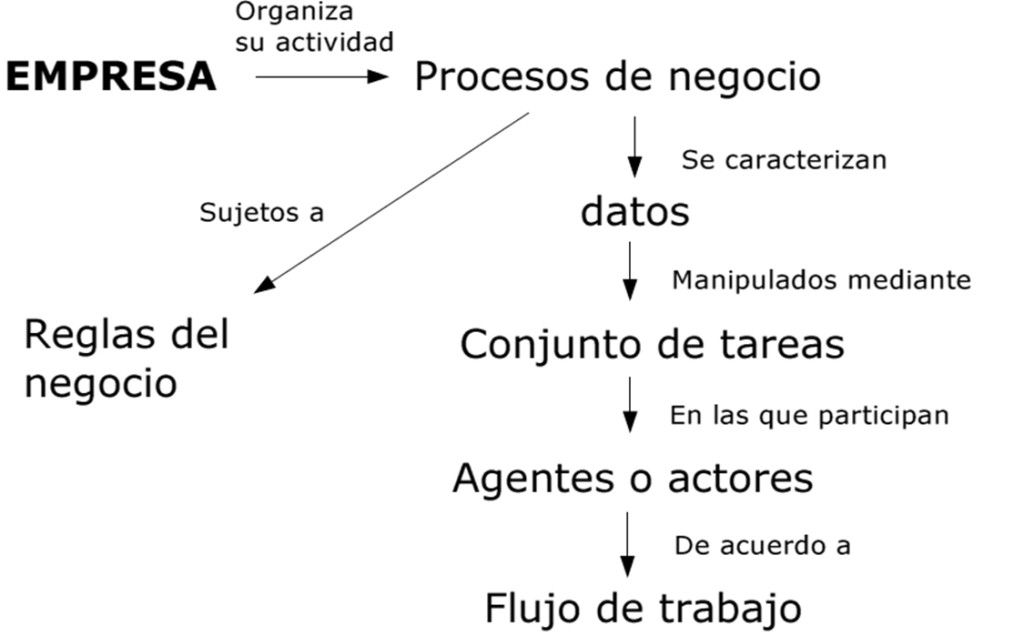
\includegraphics[width=10cm]{./Imagenes/anegocios}
\end{center}
\end{figure}

\section{Aplicacion}

Aquí va el texto.
\begin{equation}\label{eq:area}
  S = \pi r^2
\end{equation}
Uno puede referirse a ecuaciones así: ver ecuación (\ref{eq:area}).
También se pueden mencionar secciones de la misma forma: ver sección
\ref{sec:nada}. O citar algo de la bibliografía: \cite{Cd94}.



\subsection{Aplicaciones de BuBusiness Intelligence } \label{sec:nada}
\subsection{Subsection}\label{sec:nada}

Las herramientas de inteligencia de negocio son aplicaciones digitales diseñadas para colaborar con el Business Intelligence durante el análisis y la presentación de datos.\\
La Inteligencia de Negocios o Business Intelligence (BI) permite a las compañías contar con la información adecuada para una mejor toma de decisiones.  Las compañías que implementan el BI logran sacar mayor provecho de las situaciones de crisis gracias a la posibilidad de contar con un análisis de mercado más acertado debido a que los datos pesados son transformados en importantes estrategias corporativas.
Actualmente, las herramientas de BI disponibles en el mercado son incontables, pero estas 20 no pueden pasar desapercibidas:

\subsubsection{Microsoft Dynamics NAV: }\label{sec:nada2} 
Especial para pequeñas y medianas empresas que buscan mejorar su competitividad.

\subsubsection{Microsoft Dynamics CRM: }\label{sec:nada2}  
Efectiva para la administración de clientes.

\subsubsection{Oracle Business Intelligence: }\label{sec:nada2} 
Una de las más completas en el mercado ya que cuenta con paneles interactivos, análisis predictivos en tiempo real, entre otros.

\subsubsection{Ultimus: }\label{sec:nada2}  
Un entorno integrado que permite compartir información entre aplicaciones.

\subsubsection{Office SharePoint Server: }\label{sec:nada2}  
Facilita el acceso a la información en cualquier momento y lugar.

\subsubsection{QlikView: }\label{sec:nada2}  
Mantiene las bases de datos al alcance de una manera sin precedentes.

\subsubsection{Microsoft Performance Point Server: }\label{sec:nada2}  
Permite supervisar, alinear y hacer un plan de negocio.

\subsubsection{Microsoft SQL Server: }\label{sec:nada2}  
Adecuada para realizar un análisis panorámico de la empresa y tomar las mejores decisiones.

\subsubsection{JetReports: }\label{sec:nada2}  
Especial para crear informes ERP.

\subsubsection{Eclipse BIRT Project: }\label{sec:nada2}  
Genera informes para aplicaciones web de código abierto.

\subsubsection{JasperReports: }\label{sec:nada2}  
Permite crear informes de rápida impresión.

\subsubsection{LogiReport: }\label{sec:nada2}  
Aplicación gratuita basada en web de LogiXML

\subsubsection{OpenI: }\label{sec:nada2} 
Aplicación web orientada al reporting OLAP.

\subsubsection{SPSS: }\label{sec:nada2}  
Programa estadístico especialmente empleado en ciencias sociales e investigaciones de mercado.

\subsubsection{Pentaho: }\label{sec:nada2}  
Incluye herramientas para generar informes, minería de datos, ETL, entre otros.

\subsubsection{RapidMiner: }\label{sec:nada2}  
Permite analizar datos a través de un entorno gráfico.

\subsubsection{Crystal Reports: }\label{sec:nada2}  
Genera informes desde bases de datos múltiples.

\subsubsection{ApeSoft: }\label{sec:nada2}  
Ofrece una interface sencilla similar a Microsoft Excel.

\subsubsection{SAS Institute: }\label{sec:nada2}  
Facilita la gestión de riesgo financiero, desarrollo de modelos de minería de datos, etc.

\subsubsection{NiMbox: }\label{sec:nada2}  
Organiza los datos de la empresa en interactivas aplicaciones.



\subsection{Aplicaciones de BuBusiness Analitycs } \label{sec:nada}
\subsection{Subsection}\label{sec:nada}

\subsubsection{Aplicacion1: }\label{sec:nada2}  

\begin{center}
\caption\textbf{HERRAMIENTAS DE BUSINESS ANALITYCS}
\end{center}
\\
\\
Toda empresa necesita un plan de negocio. Muchos emprendedores caen en la tentación de poner en marcha su negocio sin analizar nada previamente y se limitan a cruzar los dedos esperando que salga bien. Y podría ser que sí, pero lo más probable es que no.\\
Lo ideal es llevar a cabo un análisis previo pormenorizado del sector y el mercado en el que pensamos adentrarnos. Hay numerosas herramientas de análisis estratégico gratuitas que nos pueden servir para para identificar qué distingue nuestra marca del resto y elaborar un buen plan de negocio para nuestra futura empresa. Estas son algunas de ellas.  
\\
\begin{itemize}
\item Análisis PEST
\\Con esta herramienta de análisis estratégico podremos analizar el entorno en el que queremos crear o establecer nuestra empresa, negocio o proyecto. Nos permite identificar posibles cambios de escenario en nuestro sector o en la región para detectar y aprovechar posibles oportunidades de crecimiento. El nombre es un acrónimo de cuatro factores:

Políticos: estabilidad política, la posibilidad de un cambio de gobierno que de lugar a cambios en las políticas fiscales o en materia de subvenciones, posibles cambios en los tratados comerciales, existencia o no de grupos de presión.
Económicos: economía en crecimiento o en recesión, tendencia del consumo, situación de confianza o de inestabilidad, los tipos de cambio, el nivel de inflacción…
Socioculturales: hábitos sociales, cambios en los gustos o en las modas de la gente, formas de comunicación habituales, demografía, salud, valores.
Tecnológicos: tecnología actual, posibles avances, desarrollos en marcha, conocimientos, inversión en I+D, información.
Debemos analizar en qué medida cada uno de estos factores macroambientales podría influir positiva o negativamente en nuestra empresa.  
		\begin{center}
		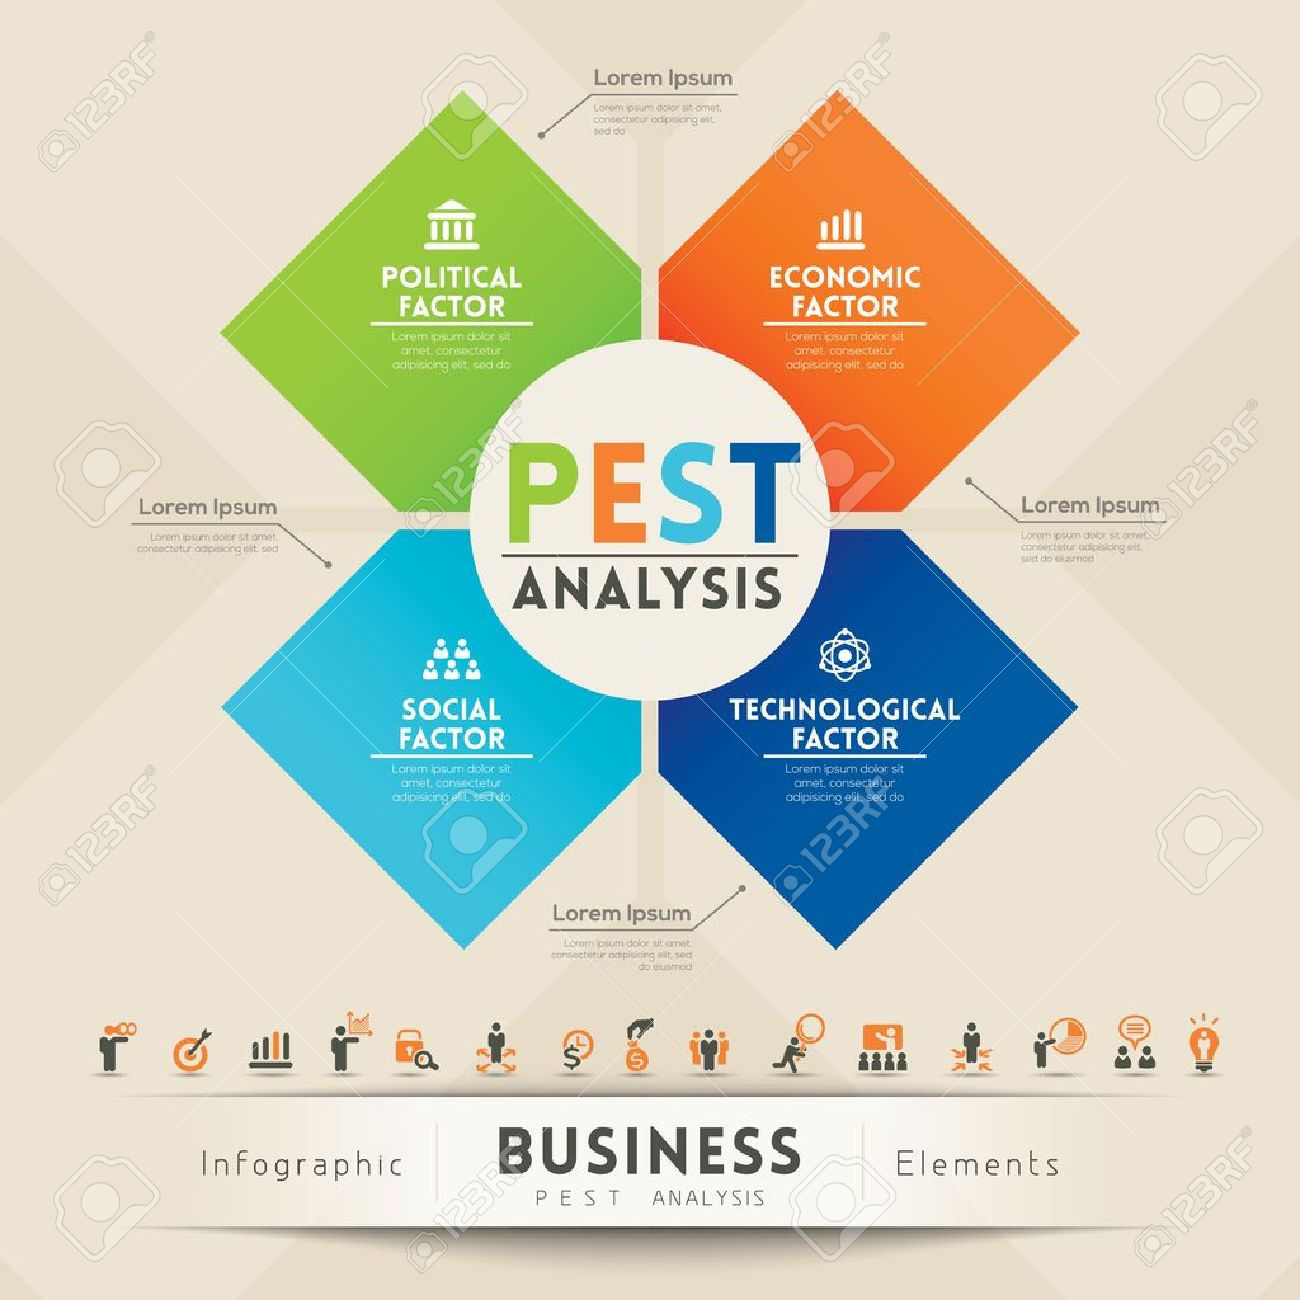
\includegraphics[width=15cm]{./Imagenes/Imagen1}
		\end{center}

	\end{itemize} 
	
	\begin{itemize}
\item Análisis PESTEL
\\Es una variación del anterior que añade dos factores más a los cuatro del análisis PEST. Además de tener en cuenta los factores políticos, económicos, sociales y tecnológicos, se analizarán también los factores:

Ecológicos: por ejemplo, el cambio climático puede tener consecuencias en diversos sectores como el turístico o el de las aseguradoras. Las leyes de protección medioambiental o las regulaciones en materia de gestión de residuos o de energías también pueden influir en una empresa.
Legales: leyes contra la discriminación, leyes de defensa del consumidor, leyes antimonopolio, licencias, legislación laboral, leyes de protección de la salud, sectores con una protección especial.
		\begin{center}
		
\includegraphics[width=15cm]{./Imagenes/Imagen2}
		\end{center}
	\end{itemize} 
  
\section{Conclusiones}
Se solía decir que la información es poder. Pero ahora el poder es entenderla. Por eso cualquier empresa hoy en día debería plantearse seriamente el uso de herramientas de análisis de datos para extraer todo el conocimiento posible de su organización. Solo así podrá mantenerse competitiva en el mercado.

(\ref{eq:area}).
También se pueden mencionar secciones de la misma forma: ver sección
\ref{sec:nada}. O citar algo de la bibliografía: \cite{Cd94}.


% Bibliografía.
%-----------------------------------------------------------------
\begin{thebibliography}{99}

\bibitem{Cd94} Autor, \emph{Título}, Revista/Editor, (año)

\end{thebibliography}

\end{document}
